\documentclass[12pt]{exam}		%Doc : https://mirrors.ircam.fr/pub/CTAN/macros/latex/contrib/exam/examdoc.pdf
\printanswers					%Comment this line to hide the answers 
\usepackage[utf8]{inputenc}
\usepackage[T1]{fontenc}
\usepackage[french]{babel}      %Originally for french document, change to english or relevant language

\usepackage{amsmath,amssymb}
\usepackage{multicol}
\usepackage[dvipsnames]{xcolor}
\usepackage[shortlabels]{enumitem}
\usepackage{tikz}
	\usetikzlibrary{fadings}
	\usetikzlibrary{calc}
	
\usepackage{tkz-tab}
\usepackage{pgfplots}

%Format Header and footer
\pagestyle{headandfoot}
\header{\footnotesize Class\\Id number}{\Large\textbf{Name}}
\headrule
\footrule
\setlength{\columnsep}{0.25cm}
%\setlength{\columnseprule}{1pt}
\footer{}{Page \thepage}{}
%\extrafootheight{-2cm}

% Change section command behaviour
\usepackage{titlesec}
\titleformat{\section}[frame]{\Huge\bfseries\filright}{}{2mm}{\centering Chemistry 123 :\ }

% Add a watermark if answers are shown
%\ifprintanswers
%\usepackage{draftwatermark}
%\SetWatermarkColor{red!30}
%\SetWatermarkScale{5}
%\SetWatermarkText{Solution}     %Watermark text
%\fi

%Format the name of each exercise
\qformat{\textbf{Exercice \thequestion~:}\hfill}
\extrawidth{1.5cm}

\begin{document}
\section{Exam 3B}

\noindent The 76 pts exam consists of 6 questions and students have the whole class period to complete the exam.
Answers must be written in the box provided or else no credit is provided. Use the empty
space provided to do your work. A periodic table is provided at the end. Fill in your name along with your
student ID number.
\\

\noindent\textbf{Problem 1: Photoelectric Effect} When light shines on a metal, electrons can be ejected from
the surface of the metal in a phenomenon known as the photoelectric effect. You perform an experiment to
eject electrons from iron (Fe) metal. It is known that a wavelength of 200 nm is the minimum energy to eject
an electron from Fe. (16 pts)
\\
\begin{enumerate}[(a)]
\item Determine the work function ($\Phi$), or the minimum energy in J to eject an electron, of the Fe metal.%
  \vspace{2in}
\item[]\tikz[baseline=1ex]\draw (0,0) rectangle (17cm,5ex);
\item How much energy in kJ is required to eject a mole of electrons from Fe metal? (Hint: One photon with
  enough energy ejects 1 electron.)
  \vspace{2in}
\item[]\tikz[baseline=1ex]\draw (0,0) rectangle (17cm,5ex);
  \newpage
\item Suppose a laser emits photons with an energy of 4.05 eV. Is this energy sufficient to eject an electron
  from Al metal? (Hint: $1 \text{ eV} = 1.602 \times 10^{-19} \text{ J}$)
  \vspace{1.75in}
\item[]\tikz[baseline=1ex]\draw (0,0) rectangle (17cm,5ex);
\item What is the velocity of the electron if a photon with a frequency $1.91 \times 10^{15} \text{ Hz}$
  hits the surface of Al metal and ejects an electron? The mass of an electron is $9.109 \times 10^{-31}$ kg.
  \vspace{1.75in}
\item[]\tikz[baseline=1ex]\draw (0,0) rectangle (17cm,5ex);
\end{enumerate}

\newpage

\noindent\textbf{Problem 2: Electron Configurations} Write the electron configuration of
the following atoms or ions. Your answer may be in the long or short forms. (12 pts)

\begin{enumerate}[(a)]
\item W
\item[]\tikz[baseline=1ex]\draw (0,0) rectangle (17cm,5ex);  
\item Ca
\item[]\tikz[baseline=1ex]\draw (0,0) rectangle (17cm,5ex);
\item P$^{3-}$
\item[]\tikz[baseline=1ex]\draw (0,0) rectangle (17cm,5ex);
\item Cu
\item[]\tikz[baseline=1ex]\draw (0,0) rectangle (17cm,5ex);
\item Al$^{3+}$
\item[]\tikz[baseline=1ex]\draw (0,0) rectangle (17cm,5ex);
\item Se
\item[]\tikz[baseline=1ex]\draw (0,0) rectangle (17cm,5ex);
\end{enumerate}

\noindent\textbf{Problem 3: Periodic Trends} Rank the following periodic trends.
(12 pts)

\begin{enumerate}[(a)]
\item Electronegativity (Strongest to Weakest): Ra, P, N, F, I
\item[]\tikz[baseline=1ex]\draw (0,0) rectangle (17cm,5ex);
\item Atomic Radius (Largest to Smallest): O, Na, Ca, Cl, Cs
\item[]\tikz[baseline=1ex]\draw (0,0) rectangle (17cm,5ex);
\item First ionization energy (Highest to Lowest): Li, Cl, Ar, He, Be  
\item[]\tikz[baseline=1ex]\draw (0,0) rectangle (17cm,5ex);
\item Electron affinity (Highest to Lowest): F, Cl, Br, I, At
\item[]\tikz[baseline=1ex]\draw (0,0) rectangle (17cm,5ex);
\end{enumerate}

\newpage

\noindent\textbf{Problem 4: Bohr's Model} The Bohr's model was first developed to explain the emission
and absorption of the hydrogen atom. (6 pts)

\begin{enumerate}[(a)]
\item What is the initial energy level of the electron if it absorbs a wavelength of 1,093 nm to a final
  energy state of 6?
  \vspace{1.75in}
\item[]\tikz[baseline=1ex]\draw (0,0) rectangle (17cm,5ex);
\item True/False. The Bohr model can accurately predict the emission and absorption of multi-electron
  atoms.
\item[]\tikz[baseline=1ex]\draw (0,0) rectangle (17cm,5ex);
\end{enumerate}

\vspace{0.3in}

\noindent\textbf{Problem 5: Classical and Quantum Pictures of Energy} Describe the difference between
the classical and quantum pictures of energy. Which theory describes that energy is quantized or
discrete steps? You may include illustrations to support your answer. (6 pts)
\vspace{0.2in}

\tikz[baseline=1ex]\draw (0,0) rectangle (17cm,55ex);

\newpage

\noindent\textbf{Problem 6: Lewis Structures and VSEPR Model} For the following compounds,
draw the Lewis structure and include resonance structures if they exist. Determine the
electronic arrangement and molecular geometry for the underlined atom. Determine whether
the molecule is polar or nonpolar. (24 pts)

\begin{enumerate}[(a)]
\item \underline{Xe}F$_4$
\item[]\tikz[baseline=1ex]\draw (0,0) rectangle (17cm,50ex);
\item CH$_3$CH$_2$\underline{C}OOH
\item[]\tikz[baseline=1ex]\draw (0,0) rectangle (17cm,50ex);
  \newpage
\item \underline{O}$_3$
\item[]\tikz[baseline=1ex]\draw (0,0) rectangle (17cm,50ex);
\item \underline{S}O$_4^{2-}$
\item[]\tikz[baseline=1ex]\draw (0,0) rectangle (17cm,65ex);
\end{enumerate}

\newpage

\appendix

\section{Apppendix 2 - Formulas and Constants}

\begin{center}
  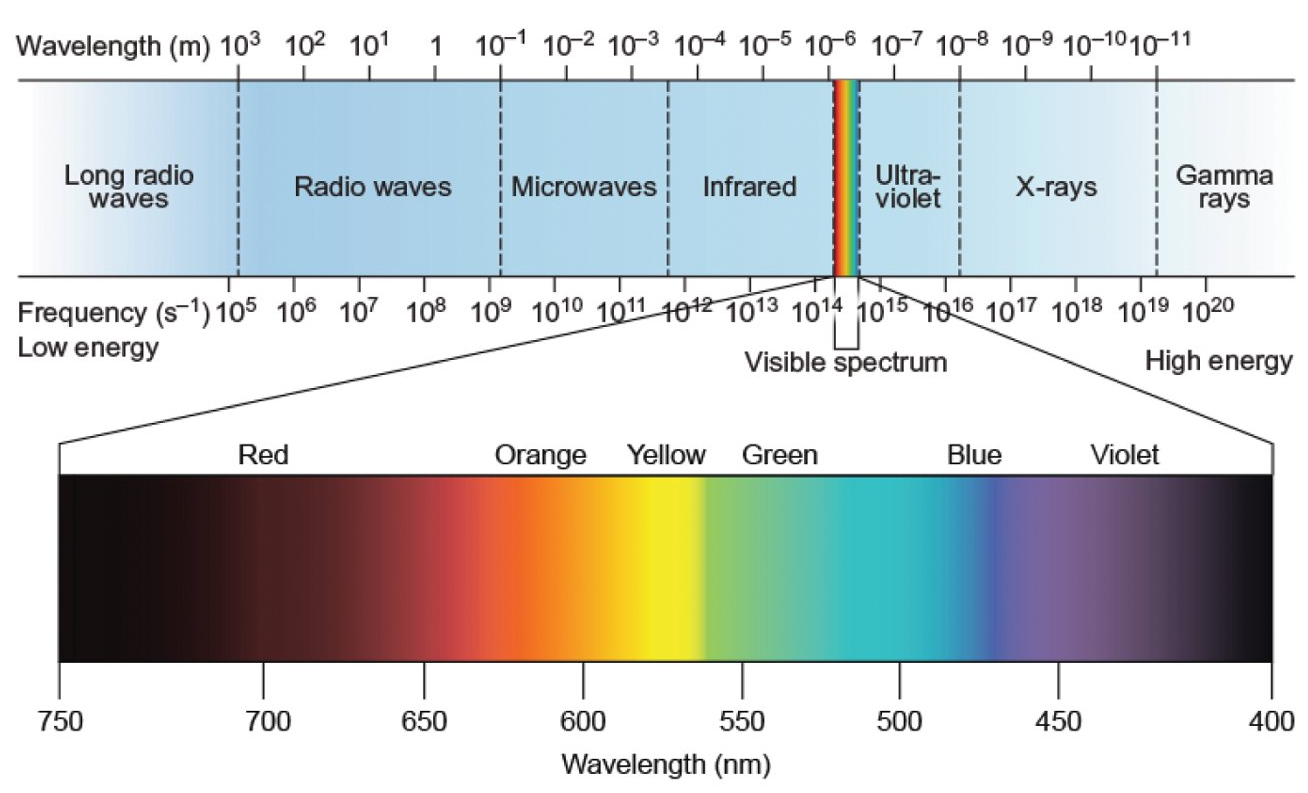
\includegraphics[scale=0.35]{electromag}
\end{center}

\begin{align*}
  c & = \lambda \nu \\
  E & = h\nu = \frac{hc}{\lambda} \\
  h & = 6.626 \times 10^{-34} \text{ J s} \\
  c & = 3.00 \times 10^{8} \text{ m/s} \\
  \text{KE} & = h\nu - \Phi \\
  \text{KE} & = \frac{1}{2} mv^2 \\
  \frac{1}{\lambda} & = R_H \Big(\frac{1}{n_1^2} - \frac{1}{n_2^2}\Big) \\
  R_H & = 1.097 \times 10^7 \text{ m}^{-1} \\
  m_\text{electron} & = 9.109 \times 10^{-31} \text{ kg} \\
  N_A & = 6.022 \times 10^{23} \text{particles/mol}
\end{align*}

\begin{center}
  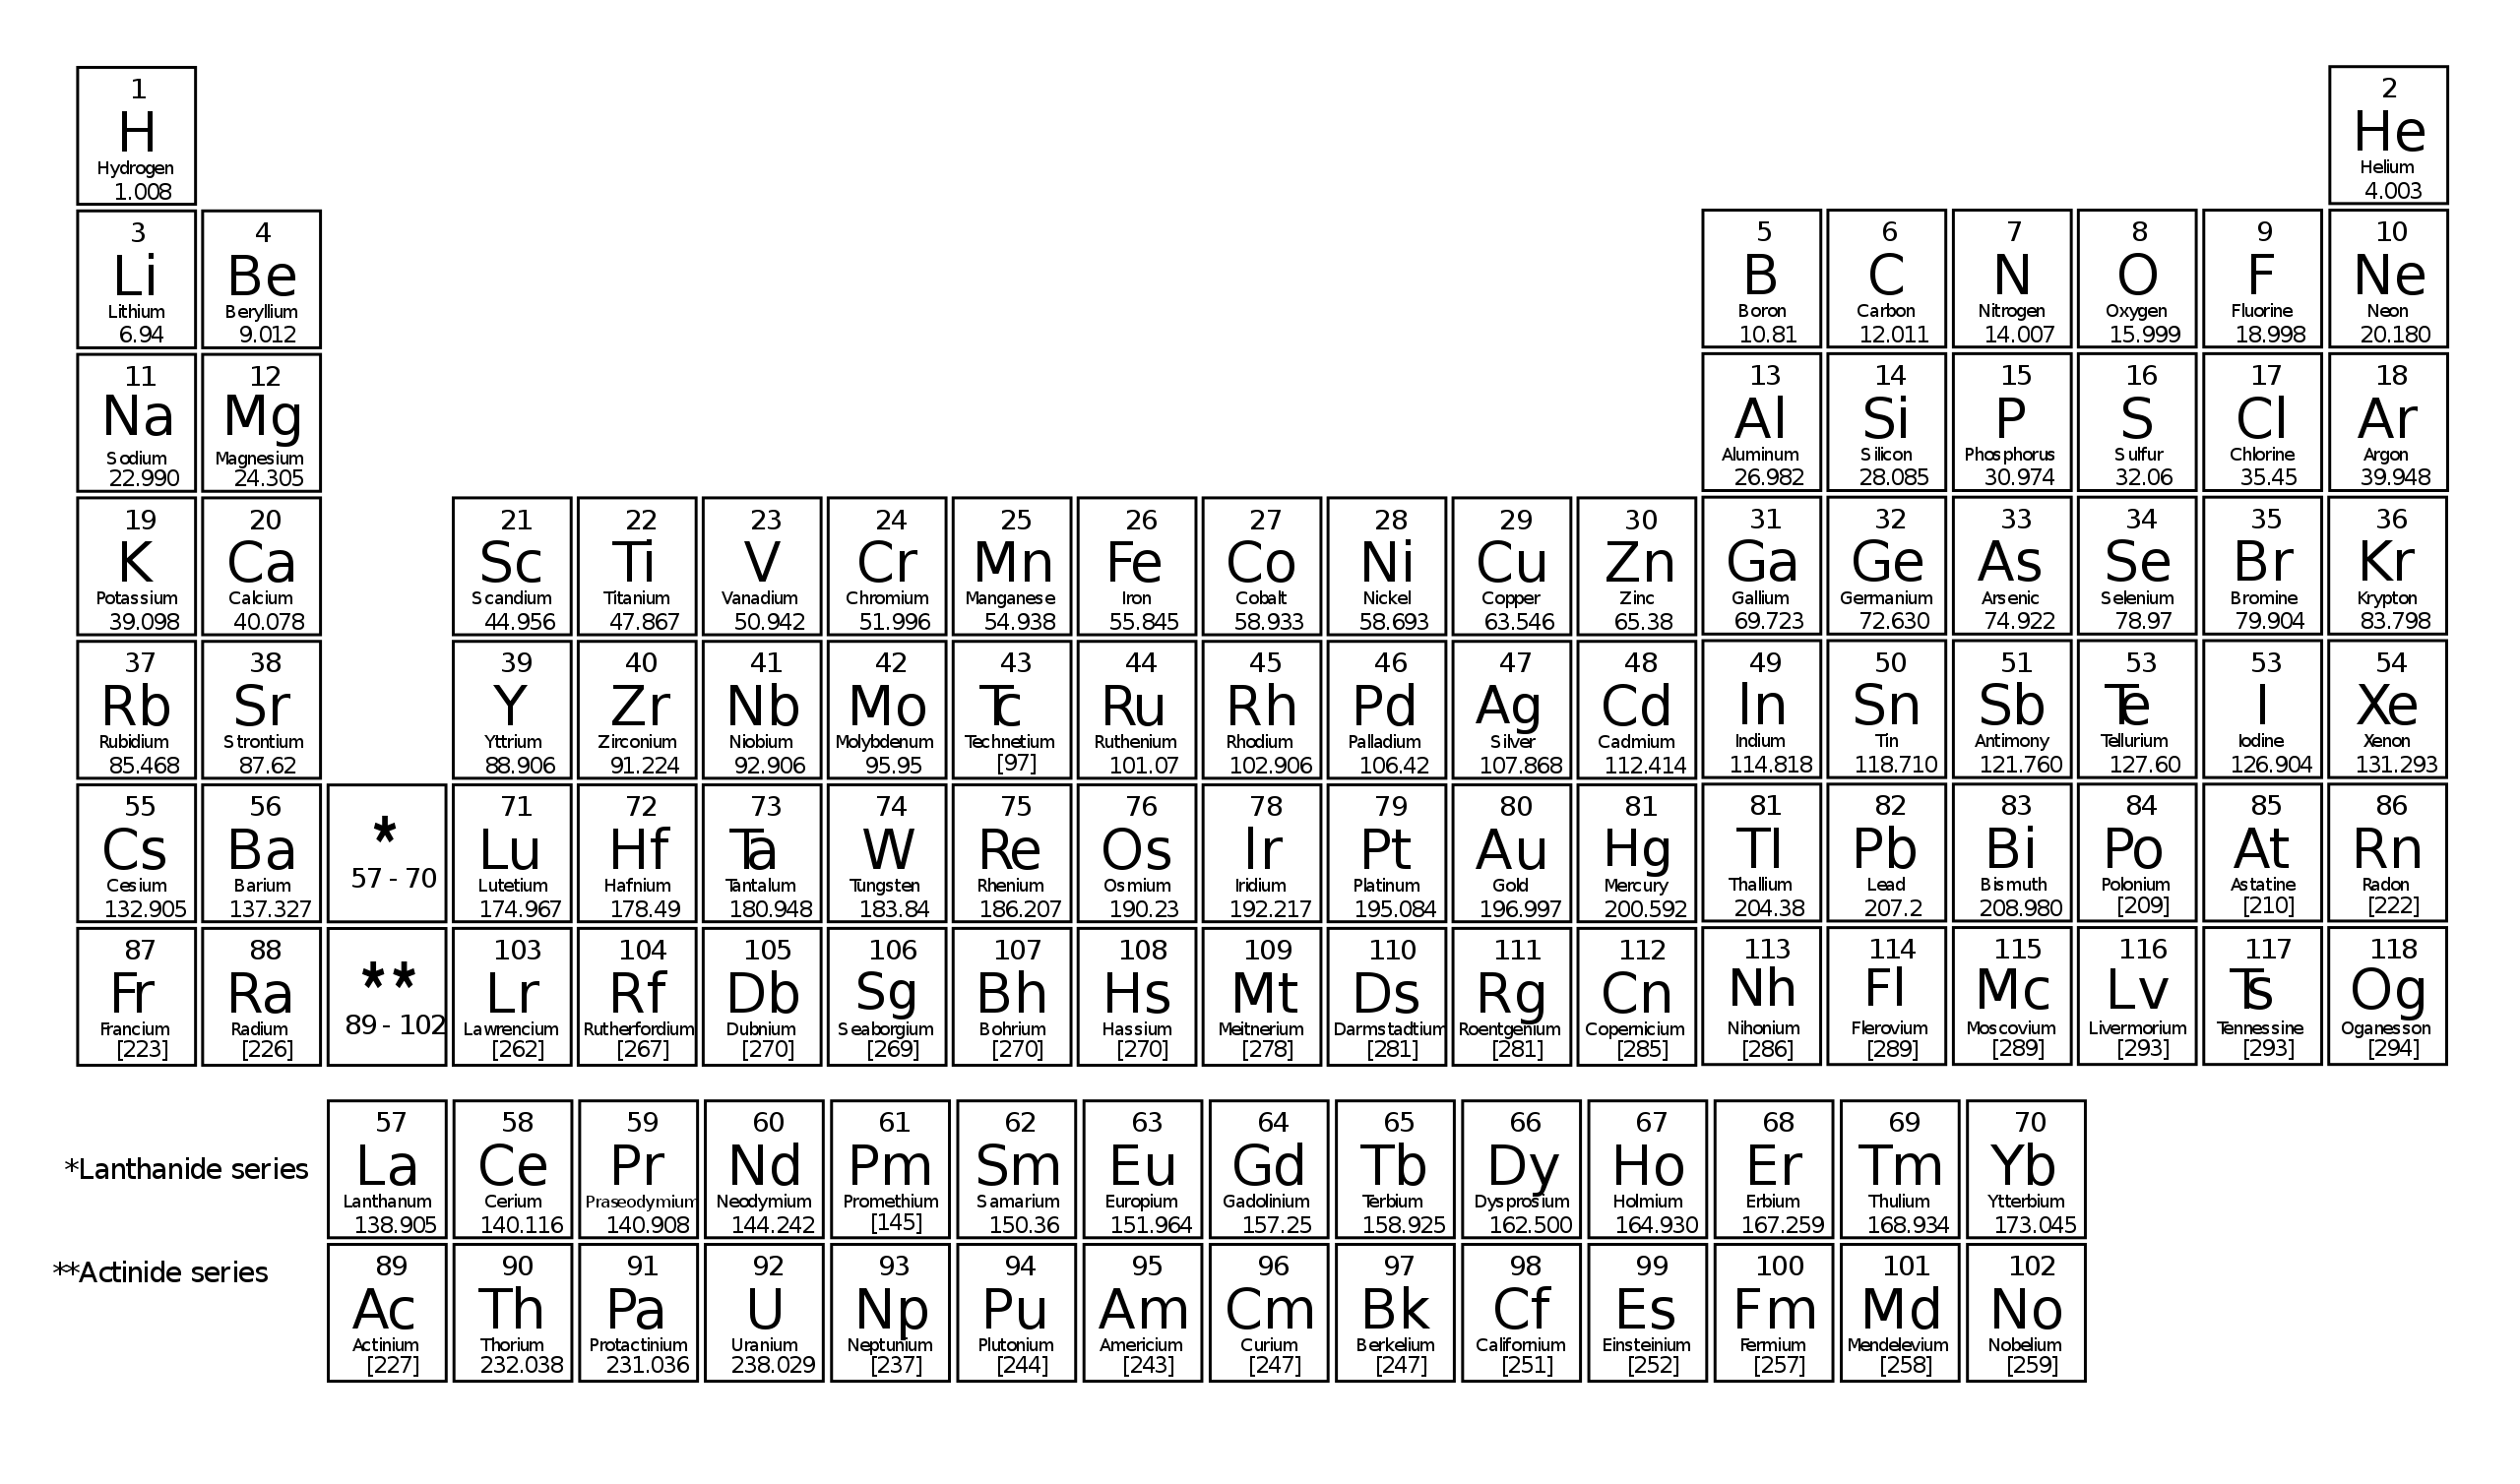
\includegraphics[scale=0.26,angle=90]{periodic_table}
\end{center}

\end{document}
